%%%% ijcai15.tex

% These are the instructions for authors for IJCAI-15.
% They are the same as the ones for IJCAI-11 with superficical wording
%   changes only.

\documentclass{article}
% The file ijcai15.sty is the style file for IJCAI-15 (same as ijcai07.sty).
\usepackage{ijcai15}
\usepackage[numbers]{natbib}
\usepackage{graphicx}
\usepackage{color}
%\usepackage{algorithmic}
\usepackage[]{algorithm2e}
\usepackage{hyperref}
\hypersetup{letterpaper,bookmarksopen,bookmarksnumbered,
pdfpagemode=UseOutlines,
colorlinks=true,
linkcolor=blue,
anchorcolor=blue,
citecolor=blue,
filecolor=blue,
menucolor=blue,
urlcolor=blue
}
\usepackage{subfigure}
\usepackage{booktabs}
\usepackage{latexsym,amssymb,amsmath} % for \Box, \mathbb, split, etc.
\newcommand{\stnote}[1]{\textcolor{blue}{\textbf{ST: #1}}}
\newcommand{\jgonote}[1]{\textcolor{green}{\textbf{JGO: #1}}}
\newcommand{\argmax}[1]{\underset{#1}{\operatorname{argmax}}\;}
\newcommand{\argmin}[1]{\underset{#1}{\operatorname{argmin}}\;}


% Use the postscript times font!
\usepackage{times}

% the following package is optional:
%\usepackage{latexsym} 

% Following comment is from ijcai97-submit.tex:
% The preparation of these files was supported by Schlumberger Palo Alto
% Research, AT\&T Bell Laboratories, and Morgan Kaufmann Publishers.
% Shirley Jowell, of Morgan Kaufmann Publishers, and Peter F.
% Patel-Schneider, of AT\&T Bell Laboratories collaborated on their
% preparation.

% These instructions can be modified and used in other conferences as long
% as credit to the authors and supporting agencies is retained, this notice
% is not changed, and further modification or reuse is not restricted.
% Neither Shirley Jowell nor Peter F. Patel-Schneider can be listed as
% contacts for providing assistance without their prior permission.

% To use for other conferences, change references to files and the
% conference appropriate and use other authors, contacts, publishers, and
% organizations.
% Also change the deadline and address for returning papers and the length and
% page charge instructions.
% Put where the files are available in the appropriate places.

\title{Bandit-Based System Adaptation for
  Instance-Based Grasping}
\author{}

\begin{document}

\maketitle

\begin{abstract}
A key aim of current research is to create robots that can reliably
manipulate generic objects.  However, in many applications,
general-purpose object detection or manipulation is not required: the
robot would be useful if it could recognize, localize, and manipulate
the relatively small set of specific objects most important in that
application, but do so with very high reliability.  The contribution
of this paper is to automate this adaptation process by formalizing a
grasping system as a hierarchy of bandit problems, enabling the robot
to apply learning techniques to adapt itself to manipulate specific
objects with increased accuracy.  The robot performs best arm
identification using a variant of Hoeffding races, enabling it to
quickly find an optimal arm and then move on to the next object.  Our
approach also incorporates knowledge from a prior defined in terms of
an ordering on the arms.  We demonstrate that our the bandit-based
adaptation step significantly improves accuracy over a non-adaptive
system, enabling a robot to quickly and autonomously acquire models
for objects, and adaptively improve them through experience.


%%   To address this
%% problem, we focus not on {\em category-based} manipulation (pick up
%% any mug) but rather {\em instance-based} manipulation (pick up this
%% mug).  

%% Our framework runs on an unmodified Baxter
%% robot; using our algorithm, a robot can interact with an object for
%% twenty minutes, and then reliably and quickly localize it with vision
%% and pick it up with closed-loop visual servoing. 

%% Instance-based recognition and pose estimation can be highly
%% accurate but require the designer to adapt the system to the specific
%% object being manipulated in large and small ways, ranging from
%% collecting training data, to choosing parameter values, to selecting
%% algorithms for tasks such as image segmentation or bounding box
%% classification.  

\end{abstract}



\section{Introduction}
Robotics will assist us at childcare, help us cook, and
provide service to doctors, nurses, and patients in hospitals. Many of
these tasks require a robot to robustly perceive and manipulate
objects in its environment, yet robust object manipulation remains a
challenging problem.  Systems for general-purpose manipulation are
computationally expensive and do not enjoy high accuracy on novel
objects~\citep{saxena08}.  Instance-based approaches that focus on
specific instances of objects can have higher accuracy but require
training by a human operator, which is time consuming and can be
difficult for a non-expert to perform~\citep{ork14, lai11, lai11a}.
Existing approaches to autonomously learn 3D object models still
require expensive ICP-based methods to localize objects, which are
susceptible to local minima and take time to
converge~\citep{krainin11}.

To address this problem, we present an approach that enables a robot
to learn to identify and grasp on a per object basis by adapting its
perceptual framework to specific objects. Our grasping and percpetion
pipeline uses standard computer vision techniques to perform data
collection, feature extraction, training, along with active visual
servoing for localization.  This framework works to some degree with
many objects, but reaches performance ceilings for specific objects
for a variety of reasons.  To address these limitations, we present a
mathematical formalization of a system of software components combined
with validators as an n-armed bandit problem~\citep{thompson33}.
Conventional abstractions and data flow used in system design
translate into independence assumptions in the model; because we are
operating using a robot which can actively collect additional
information about the environment (although sometimes at higher cost
in time and sensing), we can obtain a high-quality reward signal for
supervision.  

Unlike traditional bandit problems, where the agent trades off
exploration and exploitation, in our formulation, the robot aims to
minimize simple regret after a finite exploration
period~\citep{bubeck09}.  We follow \citet{maron93} to explore until
the agent is confident that it has found an acceptable arm.  Our
approach enables the robot to quickly converge when it finds a good
grasp, so it can move on to the next object.


%% We use slower, more accurate sensing approaches
%% to provide supervision for faster, simpler methods that excel with
%% large amounts of training data.  For example, to perform grasping we
%% use an analytic model to select grasp points, but depending on the
%% object, the best grasp according to the analytic model may not be
%% optimal; the robot can learn better grasps for that object using the
%% analytic model as a prior and actively collecting data for that
%% object.




%%  a view-based model for closed-loop visual picking.  View-based
%% methods for instance detection have many advantages over methods using
%% 3D models, because they directly capture the visual appearance of the
%% object, and are relatively simple and efficient to implement because
%% they operate on low-level features~\citep{hsiao13}.  However these
%% systems require large amounts of training data for robust performance,
%% for example more than 2000 images which must be manually collected and
%% annotated with bounding boxes for the state of the art LINE2D
%% method~\citep{hinterstoisser12}.  Moreover, for manipulation,
%% view-based methods do not propose potential grasps, and autonomous
%% methods for recognizing visual grasps are prone to error. 


%% To address these issues, we present an approach for enabling a robot
%% to train its own view-based model to recognize and manipulate the
%% specific objects it will need to use during collaborations with
%% humans.  Using our algorithm, the robot detects candidate objects for
%% training using a depth sensor, then actively collects view-based
%% visual templates to perform robust instance-based object detection,
%% pose estimation and closed-loop grasping using visual servoing.
%% Because our camera can move with seven degrees of freedom, the robot
%% can collect large quantities of data leading to simple visual models
%% that perform with high accuracy even under occlusion.  Our approach is
%% enabled by three innovations: our end-to-end algorithm for collecting
%% view-based training data with supervision obtained from a
%% higher-reliability depth sensor, which is supported by a simple and
%% robust method for determining candidate grasps using a depth sensor
%% mounted on a seven-degree-of-freedom arm, along with an approach for
%% autonomously and reliably finding object bounding boxes once the
%% object is on a background such as a floor or table.

Our evaluation demonstrates that a Baxter robot can autonomously learn
robust models for detection and grasping, using its IR sensor and arm
camera as a seven-degree of freedom one-pixel RGB-D camera.  After
training, Baxter can quickly and reliably grasp objects anywhere in
its work space using closed-loop visual servoing in response to a
person's requests.  We demonstrate that our baseline system can learn
to pick up objects approximately XX\% of the time; augmenting this
system with our self-training approach increases accuracy to YY\%.

%% Our software is compatible with ROS and the Baxter SDK version 1.0.0,
%% and we intend to release it as free software should our paper be
%% accepted.  As more and more instance-based models are collected, this
%% corpus will form a unique training set for category-based models for
%% detecting and grasping novel objects, since the robot will have a very
%% large number of views of a large set of objects as well as storing
%% depth information and grasping success.


\section{Grasping System}

We first describe our instance-based object detection and pose
estimation pipeline, which uses standard computer vision algorithms
combined to achieve a simple software architecture, a high frame rate,
and high accuracy at recognition and pose estimation.  This pipeline
can be manually trained by an expert to reliably detect and grasp
objects.  Section~\ref{sec:training} describes our approach to
enabling a robot to autonomously train this pipeline by actively
collecting images and training data from the environment using
Thompson sampling.

Our recognition pipeline takes video from the robot, proposes a small
number of candidate object bounding boxes in each frame, and
classifies each candidate bounding box as belonging to a previously
encountered object class. Our object classes consist of object
instances rather than pure object categories.  Using instance
recognition means we cannot reliably detect categories, such as
``mugs,'' but the system will be able to detect, localize, and grasp
the specific instances for which it has models with much higher speed
and accuracy.  A visualization of data flow in the pipeline appears in
Figure~\ref{fig:system}.  For each module, we formalize its input,
output, and reward function; each component can have multiple
implementations which better for different objects.  The following
sections describe how we can use this pipeline to learn which
implementation to use for specific objects; this learning dramatically
speeds up performance.

\begin{figure}
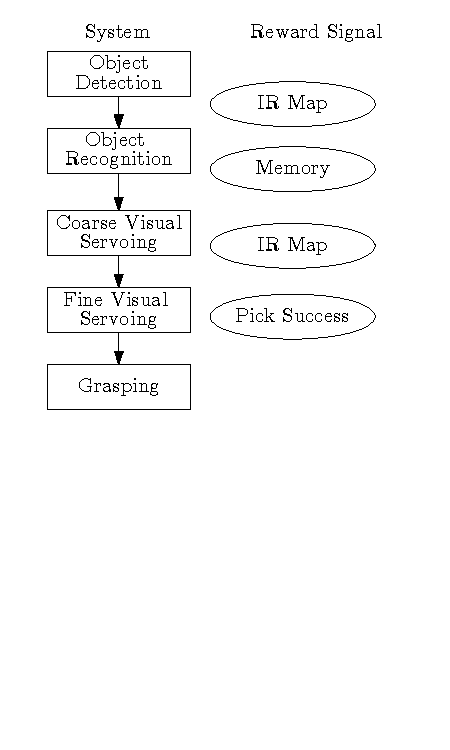
\includegraphics{system.pdf}
\caption{Data flow in our grasping system.\label{fig:system}}
\end{figure}

\subsection{Object Detection}
\label{sec:detection}

The input of the object detection component is an image, $I$; the
output is a set of candidate bounding boxes, $B$.  For object
detection we use a modified Canny algorithm which terminates before
the usual non-maximal suppression step~\citep{canny86}.

%\subsubsection{Detecting Objects Using Image Gradients}

We start by converting $I$ to YCbCr opponent color representation.
Then we apply $5 \times 5$ Sobel derivative filters~\citep{sobel95} to
each of the three channels and keep the square gradient magnitude. We
take a convex combination of the three channels, where Cb and Cr and
weighted the same and more heavily than Y.  After this we downsample,
apply the two Canny thresholds, and find connected components.  If a
connected component is contained in another, we discared the contained
component.  We throw out boxes which do not contain enough visual data
to classify.  We generate a candidate bounding box for each remaining
component by taking the smallest box which contains the component.

\stnote{Need to make a figure showing this process (analgous to the
  objectness figure)}

\subsection{Object Classification}
\label{sec:recognition}

The object recognition module takes as input a bounding box, $B$, and
outputs a label for that object, $c$, based on the robot's memory.
This label is used to identify the object and look up other
information about the object for grasping further down the pipeline.

For each object $c$ we wish to classify, we gather a set of example
crops $E_c$ which are candidate bounding boxes (derived as above)
which contain $c$. We extract dense SIFT features ~\citep{lowe99} from
all boxes of all classes and use k-means to extract a visual
vocabulary of SIFT features ~\citep{szeliski10}. We then construct a
Bag of Words feature vector for each image and augment it with a histogram of
colors which appear in that image.  The augmented feature vector is
incorporated into a k-nearest-neighbors model which we use to classify
objects at inference~\citep{szeliski10}. We use kNN because our
automated training process allows us to acquire as much high-quality
data as necessary to make the model work well, and kNN supports direct
matching to this large dataset.  

%% \jgonote{I would be careful to think about what "performing well" means to
%% us versus what it means to line2D, because I'm betting they use more objects.}
%% Existing approaches for
%% instance-based grasping such as LINE-2D require the order of $2000$ examples
%% whereas our SIFT-based approach performs well with only $200$
%% ~\citep{hinterstoisser12}.


%% The use of SIFT features is motivated by the instance level nature of
%% our task. State-of-the-art vision methods typically use
%% HOG~\citep{dalal05} features, but that choice is motivated by category
%% level recognition. \stnote{What about category level recognition
%%   motivates HOG or CNN?  Can you be more specific?}


%% is easy to rebuild online, which is a key
%% property a classifier should enjoy if it is to interact with our
%% framework in real time. State-of-the-art computer vision classifiers
%% currently employ SVM's ~\citep{} or other models which require
%% expensive training. Using such a model would introduce a training step
%% in the inside loop of our data collection process, which would be
%% costly in either engineering or time.  It is possible to use kNN
%% during the online collection process and then train a stronger
%% classifier in the background at higher latency, essentially
%% introducing a cascading step in the data collection process.

\begin{figure*}
\subfigure[Raw image from the camera.]{
  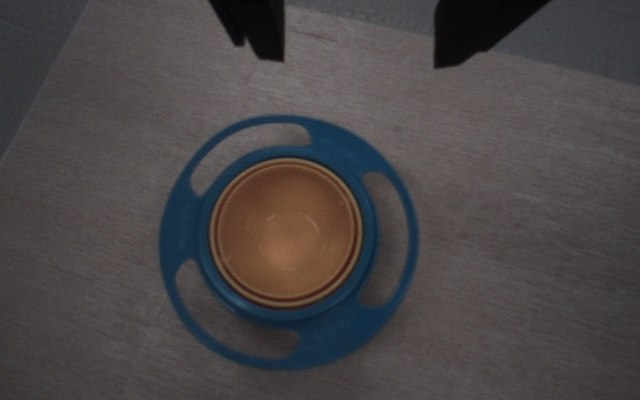
\includegraphics[width=0.25\linewidth]{figures/objectness_raw.png}}%
\subfigure[Candidate bounding boxes from Bing.\label{fig:bing}]{
  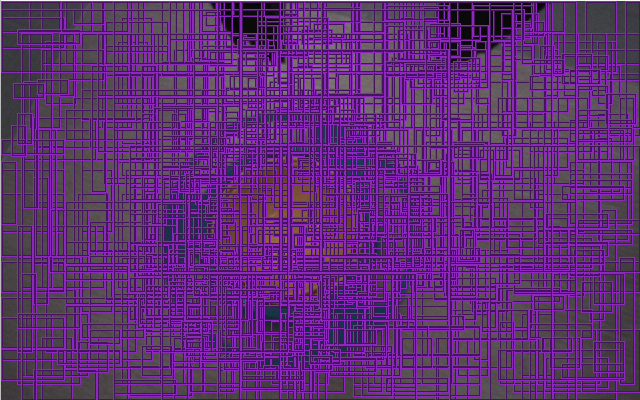
\includegraphics[width=0.25\linewidth]{figures/objectness_purple.png}}%
\subfigure[Integral image objectness map.\label{fig:objectness}]{
  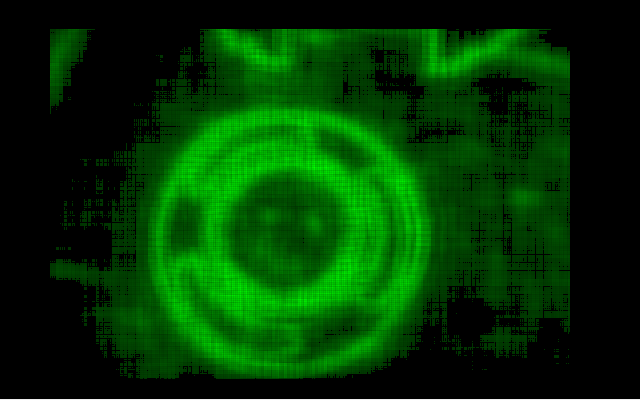
\includegraphics[width=0.25\linewidth]{figures/objectness_map.png}}%
\subfigure[Candidate bounding boxes.\label{fig:bounding_boxes}]{
  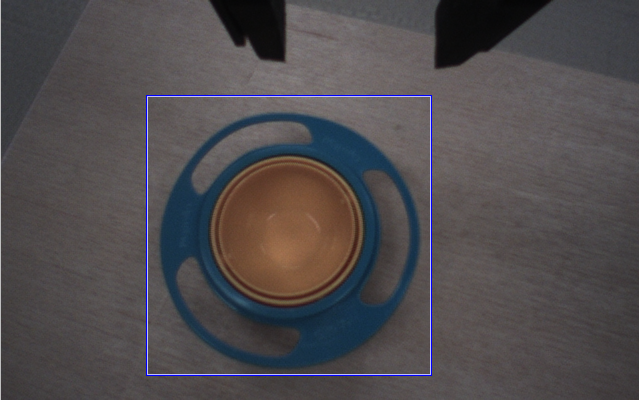
\includegraphics[width=0.25\linewidth]{figures/objectness_boxes1.png}}
\caption{The object detection pipeline, showing a raw image from the
  camera, the integral image computed using objectness, and candidate
  bounding boxes.\label{fig:object_detection}}
\end{figure*}



 
\subsection{Pose Estimation}

We use the image gradient for object detection and pose estimation. During
object detection, the gradient of the whole image is the first step in the Canny pipeline.
For pose estimation,  we require a crop of  image gradient of the object
at a specific, known pose. We denote the gradient by

\begin{align}
\Delta I = \left( \frac{\partial I}{\partial x}, \frac{\partial I}{\partial y} \right)
\end{align}

We approximate the gradient using $5 \times 5$ Sobel derivative
filters~\citep{sobel95}.  To estimate pose, we rotate our training
image and find the closest match to the image currently recorded from
the camera, as detected and localized via the pipeline in
Section~\ref{sec:detection} and~\ref{sec:recognition}.

In order to match our template image with the crop observed at pick time,
we remove the mean from and $L^2$ normalize the template and the crop.
Removing the mean provides invariance to bias, and normalizing introduces
invariance to scaling, which both help account somewhat
for lighting. 

\subsection{Identifying Grasp Points}

To identify a grasp points, we combine a depth map of the object with
a model of the gripper.  The depth map appears in
Figure~\ref{fig:depth_map}.  The grasp model scores each potential
grasp according to a linear model of the gripper to estimate grasp
success. A default algorithm picks the highest-scoring grasp point,
but frequently this point is not actually a good grasp, because the
object might slip out of the robot's gripper or part of the object may
not be visible in IR.  The input to this module is the 3d pose of the
object, and the output is a grasp point $(x, y)$; at this point we
assume only crane grasps rather than full 3d grasping.



\subsection{Closed-Loop Grasping}

To grasp an object, we first scan the work area by moving the camera
until the object is detected an recognized.  Then we perform active
visual servoing to move the arm directly above the object.  Next, we
perform orientation servoing using the pose estimation
algorithm. Because these components are instance-based, they report
position and orientation with high accuracy, enabling us to use a
proportional controller (with no derivative or integral terms) to move
the arm into position.





\subsection{Autonomous Training}
\label{sec:training}

An object model in our framework consists of the following elements:
\begin{itemize}
\item cropped object templates (roughly 200), $t^1 ... t^K$
\item depth map, $D$, which consists of a point cloud, $(x, y, z, r, g, b, d)$.
\item cropped gradient template, $t_0$
\end{itemize}

Additionally, the model can be augmented with words or attributes,
$w_1... w_n$ which people might use to describe the object, so the
robot can respond to natural language commands such as ``Put the cup
on the left table.''

To train our model, the robot first moves the object to a known pose,
then acquires images that are annotated with a pose as well as a
cropped bounding box for training.  As typical in machine learning
applications, the more images we can acquire, from the more
viewpoints, the more accurate our detection, pose estimation, and
grasping.  To achieve this accuracy, the robot autonomously collects
this information by using a depth sensor to acquire an initial grasp,
move the object to a standard known pose, and then actively collect
data for view-based methods.  Our learning algorithm appears in
Algorithm~\ref{alg:learning}.

Once the object has been moved to a known pose, we acquire the object
model by moving the camera to a sequence of prespecified orientations.
We automatically crop the image using integral images computed over
the bounding boxes inferred by the BING objectness detector.


%% \begin{figure}
%%   \textbf{GraspObject()}
%%   \begin{algorithmic}
%%     \WHILE {true}
%%       \STATE $I \gets loadImage()$
%%       \STATE $B \gets Attempt a grasp.$
%%       \IF {grasp is successful}
%%         \STATE Move object to training area.
%%         \STATE Map(object).
%%       \ENDIF
%%     \ENDWHILE
%%   \end{algorithmic}
%%   \caption{The high-level object-learning algorithm.\label{alg:learning}}
%% \end{figure}


%% \begin{figure}
%%   \textbf{Map}
%%   \begin{algorithmic}
%%     \FOR {$(x^k, y^k, z^k) \in scan$}
%%     \STATE $I^k \gets ImageAt (x^k, y^k, z^k)$
%%     \STATE $t^k \gets Crop(I^k)$ using the approach described in Section~\ref{sec:detection}
%%     \STATE $D^k \gets PointAt(x^k, y^k, z^k)$
%%     \ENDFOR
%%   \end{algorithmic}
%%   \caption{The high-level algorithm for acquiring visual and grasping
%%     models of objects.}
%% \end{figure}

\section{Bandit-based Adaptation}

Our formal model of a system defines a reinforcment learning problem,
in which the action space consists of different settings for system
parameters, and the reward function consists of the output of the
testing modules for each component.  The modular design of our system
supports a decomposition in the RL problem, so that we can treat each
optimization problem as a separate N-armed bandit problem.  In many
systems, the problem with this formulation is obtaining a reward
function to test different parameter values: the behavior of the
system must be measured by a person, and if an autonomous approach
existed to produce accurate output, it would obviate the need for the
system in the first place.  In contrast, in the robotic domain, many
edges in the system diagram can be verified, at the cost of time or
additional sensing.  This technique enables us to obtain high-quality
supervision at relevant edges in the system diagram, supporting the
decomposition into a bandit problem.  For example, optimizing grasp
height at level one is rewarded based on its accuracy at identifying
bounding boxes for the object; this training step does not require
running the entire pipeline.  Thus our algorithm for adaptation runs
from the root to the leaves of the system diagram, optimizing each
parameter based on the tester closest to it in the system tree.

Formally, the agent is given an n-armed bandit, where each arm pays
out $1$ with probability $\mu_i$ and $0$ otherwise.  The agent's goal
is to identify a good arm (with payout $>= k$) with probability $c$
(e.g., 95\% confidence that this arm is good) as quickly as possible.
As soon as it has done this, it should terminate.  The agent is also
given an ordering on the arms, promising ones first.  This order
corresponds to a prior, but the agent is only required to specific
that promising arms are first, not assign any specific probability
distribution on $\mu$.


Our algorithm is to iterate through each arm, and try it until we have
identified it either is above $k$ with probability $c$ (in which case
it terminates) or it is below $k$ with probability $c$ (in which case
it moves to the next arm in the sequence.  To compute this probability
we need to estimate the probability that the true payout probability,
$\mu$ is greater than the threshold, $c$ given the observed number of
successes and failures:
\begin{align}
\Pr(\mu_i > c|  S, F)
\end{align}

We can compute this probability using the law of total probability:
\begin{align}
\Pr(\mu_i > c|  S, F) &= \int_k^1 \Pr(\mu_i=\mu | S, F) d\mu\\
\intertext{We assume a beta distribution on $\mu$:}
                      &= \int_k^1 \mu^S (1- \mu) ^F d\mu
\end{align}

This integral is the CDF of the beta distribution, and is called the
regularized incomplete beta function~\citep{olver10}. 

\begin{algorithm}
\SetKwFunction{BestArmConfidence}{BestArmConfidence}
\BestArmConfidence{$armOrder$, $\delta$, $k$}


$\mbox{Initialize } S_0 \dots S_n \mbox{ to } 0$\\
$\mbox{Initialize } F_0 \dots F_n \mbox{ to } 0$\\
\For {$i \in armOrder$}{
  $r \gets sample(arm_i)$\\
  \If {$r = 1$}{
    $S_i  \gets S_i + 1$
  } \Else {
    $F_i  \gets F_i + 1$
  }
  $p_{reject} \gets \int_0^k Pr(\mu_i = u | S_i, F_i) d\mu $\\
  $p_{accept} \gets 1 - p_{reject}$\\
  \uIf {$p_{reject} \ge  k$} {
    break \tcp*[r]{go to the next arm}
  } \uElseIf {$p_{accept} \ge k$} {
    return $i$ \tcp*[r]{accept this arm}
  } \Else {
    pass \tcp*[r]{keep pulling this arm}
  }
}

\caption{Algorithm for Best Arm Identification\label{alg:bandit}}
\end{algorithm}




%% * terminate fast, and know when to terminate
%% * identify the best grasp with high probability (and search longer if you haven't)
%% * providing a prior
%% * providing a bound on mu. 




\section{Robotic Implementation}

We use stock Baxter and one computer.  We use the wrist cameras to
obtain RGB at 30hz. Different parts of the visual pipeline run at
different frequencies, but the full visual system runs at 2Hz in
typical conditions.  To obtain the 3D point cloud maps, we use the IR
sensor in conjunction with the RGB measurement.  Color triangulation,
a nice image of the brush.  Quickly describe raster scan.  Parzen
kernel density estimator, downsampling to fill in data.

Figure: A nice scan of the brush together with an RGB image of the brush from a similar height.


 
\section{Evaluation}

The aim of our evaluation is to assess the ability of the system to
acquire visual models of objects which are effective for grasping and
object detection.  We have implemented our approach on the Baxter
robot, which is equipped with a seven-degree-of-freedom arm with a
camera and IR depth sensor, which we use as a one-pixel depth camera
to acquire our models.

The robot acquired visual and RGB-D models for N objects using our
autonomous learning system.  We manually verified that the scans were
accurate, and set the following parameters: height above the object
for the IR scan (to approximately 2cm); this height could be acquired
automatically by doing a first coarse IR scan following by a second IR
scan 2cm above the tallest height, but we set it manually to save
time.  Additionally we set the height of the arm for the initial servo
to acquire the object.

After acquiring visual and IR models for the object at different poses
of the arm, the robot performed the bandit-based adaptation step using
Algortihm~\ref{alg:bandit}.

We report the performance of the robot at picking using the learned
height for servoing, but without grasp learning, then the number of
trials used for grasp learning by our algorithm, and finally the
performance at picking using the learned grasp location.

Our algorithm used an accept threshold of $0.7$, reject confidence of
$0.95$ and epsilon of $0.2$.  These parameters result in a policy that
rejects a grasp after one failed try, and accepts if the first three
picks are successful.  Different observations of success and failure
will cause the algorithm to try the grasp more to determine the true
probability of success.  The policy for exploring an arm appears in
Figure~\ref{fig:policy}.

\begin{figure}
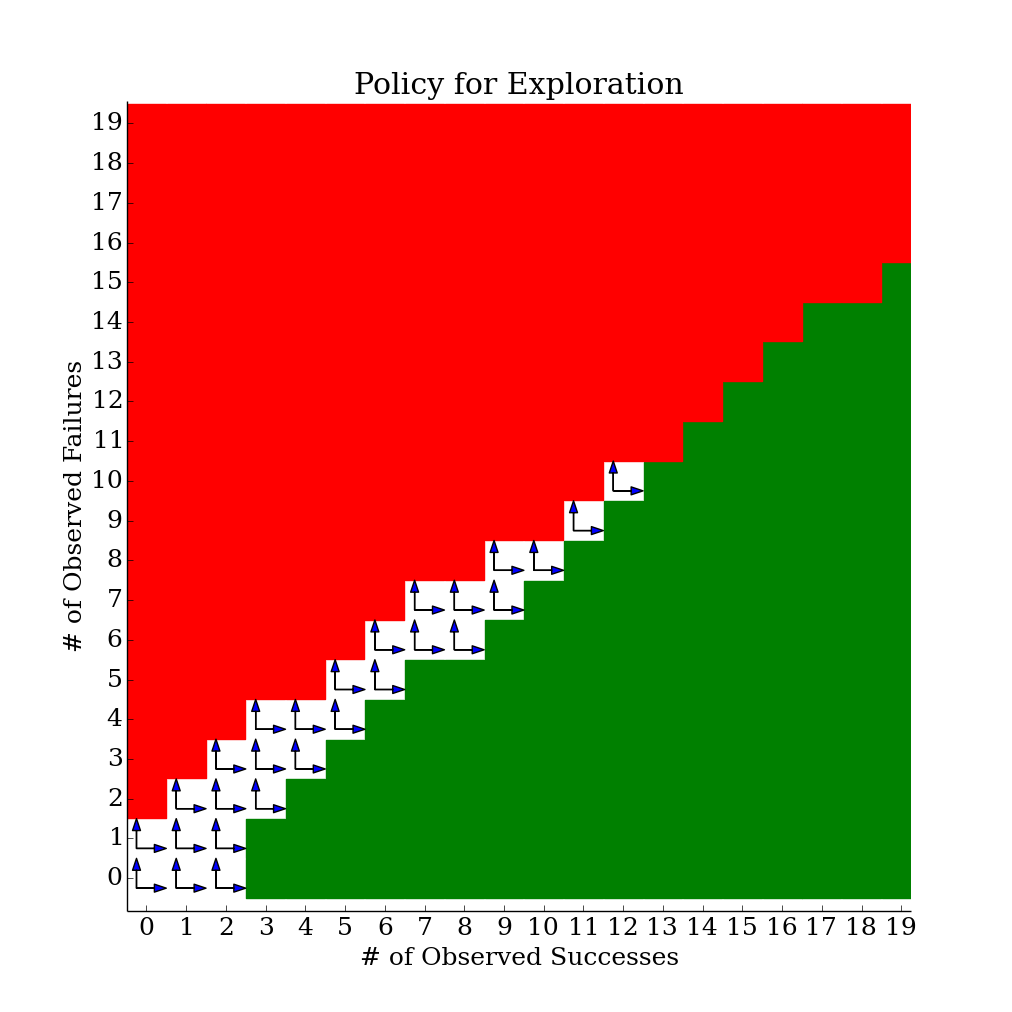
\includegraphics[width=1\linewidth]{figures/policy.png}
\caption{Policy for the agent given a belief state, defined by an
  observed number of succeseses and failures on that arm for our model
  parameters.  Red shows states where the agent rejects the arm and
  move to the next one; green shows states where it accepts the arm
  and stops learning, and the arrows show movement to the next belief
  state based on whether the next trial is successful.}
\end{figure}

\begin{table}
\begin{tabular}{cccc}
\toprule
                & Prior         &  Training     & Marginal\\
\midrule
Epipen          & 8/10          &  4/5          & 8/10 \\
Toy Egg         & 8/10          &  4/5          & 9/10 \\
Vanilla         & 5/10          &  4/5          & 9/10 \\
Triangle block  & 0/10          &  3/13         & 7/10 \\
Metal pitcher   & 6/10          &  7/12         & 10/10\\
Helicopter      & 2/10          &  8/39         & 3/10 \\
Salt shaker     & 1/10          &  4/16         & 9/10 \\
Clear pitcher   & 4/10          &  3/4          & 4/10 \\
Gyro bowl       & 0/10          &  5/15         & 3/10 \\
Sippy cup       &               &               & 4/12 \\
\midrule
Total           & 29/60         &  30/79        & 46/60\\
\bottomrule
\end{tabular}
\end{table}


\section{Related Work}

\citet{bohg13} survey data-driven approaches to grasping.  Our
approaches can be thought of as a pipeline for automatically building
an experience database consisting of object models and known good
grasps, using analytic approaches to grasping unknown objects to
generate a grasp hypothesis space and bandit-based methods for trying
grasps and learning instance-based distributions for the grasp
experience database.  In this way our system achieves the best of both
approaches: models for grasping unknown objects can be applied; when
they do not fail, the system can automatically recover by trying
grasps and adapting itself based on that specific object. 

\citet{ude12} described an approach for detecting and manipulating
objects to learn models.  It uses a bag of words model and learns to
detect the objects.  It does not learn a model for grapsing.
\citet{schiebener13} describes an extension that also does model
learning.  The robot pushes the object and then trains an object
recognition system.  It does nto use a camera that move and does not
grasp.
\citet{schiebener12} discovers and grasps unknown objects.

Summary: 
\begin{itemize}
\item People doing SLAM.  \citet{wang07, gallagher09}, 
\item People doing 3d reconstruction.   \citet{krainin11, banta00}
\item People doing big databases for category recognition.  \citet{kent14a, kent14, lai11a, goldfeder09}
\item Object tracking in vision (typically surveillance).
\item POMDPs for grasping.  \citet{platt11, hsiao10}
\item People doing systems.  \citet{hudson12, ciocarlie14}
\end{itemize}




Crowd-sourced and web robotics have created large databases of objects
and grasps using human supervision on the web~\citep{kent14a, kent14}.
These approaches outperform automatically inferred grasps but still
require humans in the loop.  Our approach enables a robot to acquire a
model fully autonomously, once the object has been placed on the
table.

\citet{zhu14} created a system for detecting objects and estimating
pose from single images of cluttered objects.  They use KinectFusion
to construct 3d object models from depth measurements with a
turn-table rather than automatically acquiring models.

\citet{chang12} created a system for picking out objects from a pile
for sorting and arranging but did not learn object models.  

next-best view planning~\citep{kriegel11}

\citet{nguyen14} learn to manipulate objects such as a light switch or
drawer with a similar self-training approach.  Our work learns visual
models for objects for autonomous pick-and-place rather than to
manipulate objects.

Developmental/cognitive robotics~\citep{lyubova13, kraft10r}

\citet{banta00} constructs a prototype 3d model from a minimum number
of range images of the object.  It terminates reconstruction when it
reaches a minimum threshold of accuracy.  It uses methods based on the
occluded regions of the reconstructed surfice to decide where to place
the camera and evaluates based on the reconstruction rather than pick
up success.  \citet{krainin11} present an approach for autonomous
object modeling using a depth camera observing the robot's hand as it
moves the object.  This system provides a 3d construction of the
object autonomously.  Our approach uses vision-based features and
evaluates based on grasp success.  Eye-in-hand laser
sensor.~\citep{aeotti14}

\stnote{Need to find the instance-based work that Erik mentioned when
  he said it was a ``solved problem.''}

\citet{velez11} created a mobile robot that explores the environment
and actively plans paths to acquire views of objects such as doors.
However it uses a fixed model of the object being detected rather than
updating its model based on the data it has acquired from the
environment.

Methods for planning in information space \citep{he08, atanasov13,
  prentice09} have been applied to enable mobile robots to plan
trajectories that avoid failures due to inability to accurately
estimate positions.  Our approach is focused instead on
object detection and manipulation, actively acquiring data for use
later in localizing and picking up objects. \stnote{May need to say
  more here depending on what GRATA actually is.}


Early models for pick-and-place rely on has been studied since the
early days of robotics~\citep{brooks83, lozano89}.  These systems
relied on models of object pose and end effector pose being provided to the
algorithm, and simply planned a motion for the arm to grasp.  Modern
approaches use object recognition systems to estimate pose and object
type, then libraries of grasps either annotated or learned from
data~\citep{saxena08, goldfeder09, morales03}.  These approaches
attempt to create systems that can grasp arbitrary objects based on
learned visual features or known 3d configuration.  Collecting these
training sets is an expensive process and is not accessible to the
average user in a non-robotics setting.  If the system does not work
for the user's particular application, there is no easy way for it to
adapt or relearn.  Our approach, instead, enables the robot to
autonomously acquire more information to increase robustness at
detecting and manipulating the specific object that is important to
the user at the current moment.

Visual-servoing based methods~\citep{chaumette06} \stnote{Need a whole
  paragraph about that. }

\stnote{\citet{ciocarlie14} seems highly relevant, could not read from
  the train's wifi.}  Existing work has collected large database of
object models for pose estimation, typically curated by an
expert~\citep{lai11}.  \citet{kasper12} created a semiautomatic system
that fuses 2d and 3d data, but the setup requires a special rig
including a turntable and a pair of cameras.  Our approach requires an
active camera mounted on a robot arm, but no additional equipment, so
that a robot in the home can autonomoulsy acquire new models.

\citet{collect14} describes an approach for lifelong robotic object
discovery, which infers object candidates from the robot's perceptual
data.  This system does not learn grasping models and does not
actively acquire more data to recognize, localize, and grasp the
object with high reliabilitiy.  It could be used as a first-pass to
our system, after which the robot uses an active method to acquire
additional data enablign it to grasp the object.  Approaches that
integrate SLAM and moving object tracking estimate pose of objects
over time but have not been extended to manipulation~\citep{wang07,
  gallagher09, salas-moreno13, selvatici08}.

Our approach is similar to the philosphy adopted by Rethink Robotic's
Baxter robot, and indeed, we use Baxter as our test
platform~\citep{fitzgerald13}.  \stnote{Haven't actually read this
  paper, just making stuff up based on Rod's talks.  Should read the
  paper and confirm.}  Baxter's manufacturing platform is designed to
be easily learned and trained by workers on the factory floor.  The
difference between this system and our approach is we rely on the
robot to autonomously collect the training information it needs to
grasp the object, rather than requiring this training information to
be provided by the user.


Robot systems for cooking~\citep{bollini12, beetz11} or furniture
assembly~\citep{knepper13} use many simplifying assumptions, including
pre-trained object locations or using VICON to solve the perceptual
system.  We envision vision or RGB-D based sensors mounted on the
robot, so that a person can train a robot to recognize and manipulate
objects wherever the robot finds itself.

Approaches to plan grasps under pose uncertainty~\citep{stulp11} or
collect information from tacticle sensors~\citep{hsiao10} using
POMDPs.  \citet{plat11} describe new algorithms for solving POMDPs by
tracking belief state with a high-fidelity particle filter, but using
a lower-fidelity representation of belief for planning, and tracking
the KL divergence.

\citet{hudson12} used active perception to create a grasping system
capable of carrying out a variety of complex tasks.  Using feedback is
critical for good performance, but the model cannot adapt itself to
new objects.



\section{Conclusion}

\stnote{First paragraph:  contributions.  What are the things this paper has done to advance the state of the art?}

\stnote{Next paragraphs: future work, spiraling upward to more and
  more ambitiuos extensions.}

Right now, NODE runs on Baxter. We will port NODE to PR2 and other AH systems.
GRATA could be applied in other domains as well.  What are some examples?

Ideas for doing for the paper, otherwise future work: 
\begin{itemize}
\item Semantic mapping. 
\item Detection and manipulation in clutter and occlusion.
\item Amazon mechanical turk for labels, so we can follow commands and gesture.
\item Object tracking over time so we can answer questions about what
  happened to the object.
\item Object oriented SLAM so we can handle joint localization and mapping.
\item Semantic mapping of objects over time.  Deciding when to go look
  again, maintaining history, etc. 
\item Scaling to lots and lots of objects.
\item Using the database of lots and lots of objects to do category recognition.
\item Multiple poses during training (e.g., what happens when you drop
  the object?)
\end{itemize}


%% The file named.bst is a bibliography style file for BibTeX 0.99c
{\tiny
\bibliographystyle{plainnat}
\bibliography{main,references}
}
\end{document}

